\chapter{Reinforcement-Learned Balancing}
\label{chap:ns}

\section{Introduction}

A major goal of the RoboCup Standard Platform League is the development of improved bipedal control of the Nao robots. The teams aim to demonstrate that the robots are able to execute increasingly human-like bipedal behaviours, whether it be walking, kicking a ball, or self-stabilisation. The ability to execute these types of movements, to be able to switch between them fluidly, and to react against external forces to avoid falling over is a key research area in robotics. The responsiveness required by such movements is what is to be expected of future robots particularly when emulating human behaviours, as in playing a game of soccer.

Such behaviour is extremely difficult or practically impossible to be programmed directly into a robot. Careful study and analysis of human movement is required and mathematical models must be derived to approximate it. Even then, such models tend only to work in ideal situations, such as walking over a perfectly smooth and flat ground. In order to approach the behaviour that is inherent in humans -- that of adapting to any possible situation -- it is necessary that machine-learning principles are considered in order to adapt to any change in the robot's environment. For example, a hand-programmed walk will react differently over a rough and bumpy surface than over a flat and smooth surface, as it is confined to a small subset of possible robot states, whereas a machine-learned walk should in theory be able to react to either.

For the 2013 Open Challenge, we explored the application of Reinforcement-Learned behaviours for bipedal movements on the Nao robots. We aimed to demonstrate that simulator-learned behaviours could be applied directly to the Nao robots without the need for significant tuning in software. The Open Challenge entry was titled \textit{``Stability Control through Machine Learned Behaviours''}\cite{openchallenge}.

The learned behaviours aimed to react to a greater number of states than hand-programming would allow for and to allow relatively simpler implementation of more advanced behaviours. Applied to the Naos, we aimed for self-stabilisation without the need for hard-coding in a variety of states including: changing support feet at different frequencies (walking on the spot); standing upright; standing on either foot; and seamlessly switching between these. 

\newpage
\section{Background \& Related Work}

Reinforcement Learning (RL) is a method of deriving software models for behaviour through machine learning. RL is used to automatically determine a model for actions to be taken given an ``environment state'' such that the maximum ``reward'' can be achieved. In the context of stability control for bipedal robots, RL results in a software model (known as a \textit{policy}) which states what motors the robot should actuate and in what manner, given that the robot is in some state (the environment state) and wants to reach some position (the reward).

An RL model is defined by:\cite{bernhard_rl}

\begin{description}
\item[States] -- the set of all states the robot can be expected to act in.
\item[Actions] -- the set of all actions the robot can potentially take.
\item[Transitions] -- the definition of how states transition into other states.
\item[Reward] -- the definition of how good being in a certain state or doing a certain action is.
\end{description}

%The Q-learning -> learns to assign values to (s,a) pairs.
%Given a particular action in a particular state, followed by actions which follow a particular policy, the agent will receive a particular set of reinforcement.

RL works by finding a function which gives the value of taking a particular action when in a particular state and then following the optimal policy thereafter. The optimal value is therefore the best one of the possible actions that can be taken at a given state. The ``value'' of each state-action is dependent on the reward -- taking actions which lead to rewards quickly is of higher value, taking actions which lead to slow or negative rewards is of lower value.

The work presented in this report relies primarily on the application of RL research done by Hengst\cite{bernhard_rl}. Hengst's work involved the use of a simulated environment for the robot, allowing for fast reinforcement learning of optimal policies for various behaviours (defined by their cost (inverse of reward) functions), including:

\begin{itemize}
\item Standing upright and still.
\item Standing on one leg.
\item Rocking between both legs.
\end{itemize}

Hengst's work allows for a much simpler implementation of the policies in real hardware with less need for learning or tuning on the hardware. Testing this is one of the primary aims of the work outlined in this report.

White's\cite{white} 2011 implementation of a simulator-learned policy for a walking gait on the Naos is also an important motivator. White was able to show that a simulator-learned walk running on the Naos was able to react to obstacles significantly better than one with no RL policy. However, White also found that state measurement was very difficult due to noisy sensors and limited data, and the work was not merged into the competition code.

Further work by Liu\cite{liu} in 2012 focused primarily on improving state measurement by introducing heavy filtering of the Inertial Measurement Unit (IMU) located in the chest of the Naos. While the demonstrated filters worked well, Liu found that the underlying assumptions in the filter (that the robot is standing still, upright, and approximates an inverted pendulum) were not sufficient when introducing more complex motion such as a walking gait.

\section{Theory \& Implementation}

\subsection{RL Policies}
In learning the policies for the behaviours, Hengst\cite{bernhard_rl} defines a robot model, including as much accuracy in the links, joints, masses, etc. as possible -- an example of this is seen in Figure \ref{fig:lean}. Hengst defined the robot stabilisation state and established cost functions in the form of goal behaviours (such as standing upright), and state transitions as random action exploration, able to automatically identify the system model (i.e. it did not assume an inverted pendulum model). 

\begin{figure}[h]
\centering
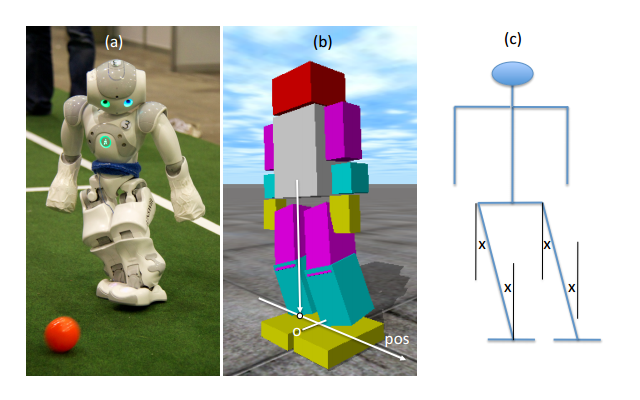
\includegraphics[width=3.5in]{img/RL_lean.png}
\caption{The Nao robots modelled as a $23 DOF$ (Degree of Freedom) system in (b). \cite{bernhard_rl}}
\label{fig:lean}
\end{figure}

Hengst's work calculated the transition function between states by observing the state changes in the simulation of the robots when subjected to a random choice of actions (from the set of actions that could be taken) -- the random simulation essentially explored the state space of the model through the actions. This is considered a time-consuming process and is a practically impossible task to achieve using real-life hardware tests (due to the complexity in analysing the environment, something a simulation can do very easily). This state exploration could take several hours to calculate, depending on the desired resolution of states.

Once the state transitions were known (to whatever degree), it was a simple case of calculating the value of each state-action for any given reward function, and then finding the optimal action to take for a given state-action (that is to say, the action to take depends not only on the current state, but also on the previous action taken). The list of optimal actions for each state-action is then known as the \textit{optimal policy}. A reward function could be easily created for any goal desired, such as standing still or walking on the spot, so long as the goal states were in the set of explored states. Knowing the state transitions also allowed for quick switching between behaviours by simply picking which policy to follow.

The optimal policy for any behaviour could then be given as a simple output of numbers, simply being the state-action pair and the corresponding optimal action to take. An excerpt from a policy can be seen below:


\newcommand\statehighlight[1]{\textcolor[rgb]{1,0,0}{#1}}
\newcommand\actionhighlight[1]{\textcolor[rgb]{0,0,1}{#1}}
\begin{Verbatim}[commandchars=\\\{\},frame=single]
// Policy table for 6 Coronal behaviours
// State-action is defined by: Goal, lateral torso position, 
//                             lateral torso velocity, 
//                             last action taken
// Action: 0 for ankle roll left, 1 for no action, 2 for ankle roll right
//  \statehighlight{state-action}    \actionhighlight{action}
   0 -0.08 -0.4  0     0
   0 -0.08 -0.39 0     1
   0 -0.08 -0.38 0     1
   0 -0.08 -0.37 0     2
\end{Verbatim}

\subsection{}


\subsection{Implementation}
The work done in this year was an attempt to combine the previous works of Hengst, White, and Liu in order to produce more stable 



Much of the work done is in fact an incremental improvement to White's policy implementation, as well as the application of the improved policies done by Hengst.

We begin by defining a robot model, including as much accuracy in the links, joints, masses, etc. as possible -- an example of this is seen in Figure \ref{fig:lean}. We define the robot stabilisation state and establish cost functions in the form of goal behaviours (such as standing upright, for example), and state transitions as random action exploration, able to automatically identify the system model (i.e. we do not assume an inverted pendulum model). 

The reinforcement learning then learns the actions required for optimal stabilisation of given behaviours, as well as for the transition between behaviours. These actions are used in the creation of policies, which define the action required for each possible state of the robot. Some simplified example policies can be seen in Figure \ref{fig:policy}.

The policy tables are then interpreted by the real-world Nao robots, allowing them to mimic the behaviour seen in the simulation by actuating joints to follow the optimal action sequence.

\section{Results}
For the RoboCup 2013 Open Challenge we plan to demonstrate a robot which is able to self-stabilise with various behaviours, including standing on one leg and jogging on the spot. The robot is also able to seamlessly and optimally transition between these behaviours while maintaining a stable body, something already exceedingly difficult in manual hand-coding of behaviours.

Most importantly, we plan to show the continued stability of a robot even when reacting to disturbances, such as being bumped by another robot. Given the dynamic behaviour of such disturbances, hand-coding is virtually impossible or relies on extensive trial-and-error manual tuning -- whereas this is simply a property of the learned optimal policies for any behaviour, therefore guaranteeing simple automatic stabilisation of the robots after policy learning.


Despite disappointing behaviour in the field, the presentation of the work was considered worthy of $3^{rd}$ place in the Open Challenge.


\begin{figure}[!t]
\centering
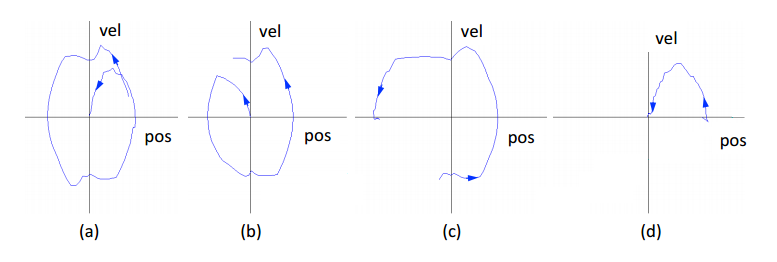
\includegraphics[width=3.5in]{img/RL_policies.png}
\caption{Simplified example of learned policies. Here we see the transition functions between the behaviours of: (a) switching between a slow walk-on-the-spot to standing upright; (b) standing upright to walk-on-the-spot; (c) walk-on-the-spot to standing on right leg; (d) standing on left leg to standing upright.}
\label{fig:policy}
\end{figure}


\section{Evaluation}
\section{Future Work}
\section{Conclusions}
